% !TEX root = ../dissertation.tex

\chapter{Mathematical Background}
This is some text
\section{Dumbbell Spacecraft Equations of Motion}\label{sec:dumbbell}

In this section we derive the equations of motion of a rigid spacecraft under the influence of the gravitational attraction of a homogenous asteroid.
The motion of a spacecraft around an asteroid is markedly different than that of Earth orbiting vehicles.
First, the gravitational field around an asteroid is highly irregular and complex. 
The usual assumption of a spherical potential is not valid for small or irregular shaped bodies.
Furthermore, since the magnitude of the gravitational attraction is relatively small, non-gravitational effects, such as solar radiation pressure or third-body effects, become much more significant.
As a result, the orbital environment is generally quite complex and it is difficult to generate analytical insights, such as the Keplerian two-body solution.

A second key consideration is the coupling between rotational and translational states around the asteroid.
The coupling is induced due to the different gravitational forces experienced on various parts of the spacecraft.
The effect of the gravitational coupling is related to the parameter \(\epsilon = \frac{r}{R_c}\), where \(r\) is the characteristic spacecraft length and \(R_c\) is the orbital radius~\cite{hughes2004}.
For Earth based missions, the orbital radius is several orders of magnitude larger than the spacecraft length and \(\epsilon\) is small.
As a result, the corresponding gravitational moment is weak and can be neglected. 
Therefore, the translational and rotational equations of motion become decoupled and can be considered separately, significantly simplifying the analysis. 
However, for operations around an asteroid the orbital radius is much smaller, which leads to much larger values of \(\epsilon\) and much larger influence of the rotational and translational coupling.
References~\cite{elmasri2005} and~\cite{sanyal2004} investigated the coupling of an elastic dumbbell spacecraft in orbit about a central body, but only considered the case of a spherically symmetric central body.

With these insights, we seek to develop the complete coupled equations of motion of a spacecraft around an asteroid.
The equations of motion should explicitly consider the interaction of the translational and rotational dynamics.
Furthermore, the equations should be defined in a global and coordinate-free representation to allow for a single global representation of the motion of the spacecraft and asteroid.

\subsection{Reference Frames}\label{ssec:dumbbell_eoms_reference_frames}

The first step in deriving the equations of motion is to first define the \gls{kinematics} of the spacecraft motion.
This kinematical description will be used in subsequent sections to simulation the motion and define the sensor measurements and asteroid reconstruction.
There are three reference frames of interest for this problem:
\begin{enumerate}
    \item \( \vecbf{e}_i \) : The inertial reference frame is assumed to be fixed in space. 
        The origin of the frame is chosen to coincide with the center of mass of the asteroid.
        The standard orthornormal basis, \( \vb{e}_1, \vb{e}_2, \vb{e}_3\) are fixed with respect to the stars.
    \item \( \vb{f}_i \) : The asteroid fixed frame is a rotating reference frame which is fixed to the surface of the asteroid.
        The reference frame originates at the center of mass of the asteroid and the basis vectors are aligned with the principle motments of inertia of the asteroid.
        In addition, we assume that at the beginning of any simulation that the asteroid and inertial frames are initially aligned.
    \item \( \vb{b}_i \) : The spacecraft fixed reference frame is attached to the spacecraft and aligned with the principle moments of inertia.
        The frame originates at the center of mass of the spacecraft.
\end{enumerate}
The reference frames are also shown in~\cref{fig:reference_frames}.
\begin{figure}
    \centering
    \includegraphics[width=\textwidth]{example-image-golden}
    \caption{Representation of the three reference frames, inertial, asteroid, and spacecraft, used to describe the kinematics\label{fig:reference_frames}}
\end{figure}

With the appropriate reference frames, the configuration space of the spacecraft motion is now defined to enable the derivation of the equations of motion.
From classical mechanics, the parameters which are used to define the motion of the system are called generalized coordinates, and the vector space defined by these coordinates is called the configuration space of the physical system.
Frequently, the physical parameters of the system must also satisfy some mathematical constraints, which then define a configuration manifold of all generalized coordinates within the configuration space which satisfy the constraints.
For example, the motion of a particle in three-dimensional Euclidean space can be defined by the typical generalized coordinates in the form of a vector
\begin{align*}
    \vb{r} = \begin{matrix}
        x_1 & x_2 & x_3
    \end{matrix}^T.
\end{align*}
Therefore the configuration space is then the set of all real three dimensional vectors or equivalently,
\begin{align*}
    \vb{r} \in \R^3.
\end{align*}
If we further assume that the point is constrained to the surface of a sphere, for example in the case of a spherical pendulum, then the configuration space becomes the subset of \( \R^3 \) which also define points the on sphere, \( \S^2 \).
If the particle is an extended body rather than a point mass then the orientation becomes an additional configuration parameter.
The orientation of any rigid body can be defined as the orientation of a body fixed reference frame with respect to an inertial frame. 
As a result, the configuration space for the general motion of a rigid body is defined by at a minimum of three coordinates to represent translation and three coordinates to represent the orientation.
This configuration space is the semi-direct product, \(\SE = \R^3 \times \SO \), or the special euclidean group.
The special euclidean group is the group of all possible rigid body motions and defines the six degrees of freedom possible by our system.
An element of the special euclidean group can be expressed using the homogenous representation as
\begin{align*}
    \begin{bmatrix}
        R & \vb{x} \\
        0 & 1,
    \end{bmatrix}
\end{align*}
where \( R \in \SO\) is a \( 3 \times 3 \) real matrix with determinant of \( +1\) and \( \vb{x} \in \R^{3 \times 1}\) is a column vector.

% TODO Discuss the group update operation as a homogenous transformation on R^4
% TODO show example of the update operation 
The variations should be carefully constructed such that they respect the geometry of the configuration space.
By expressing the motion of the dumbbell directly on the special euclidean group, we avoid the issues inherent in using other kinematic representations which fail to preserve the geometric properties of the configuration space.
The kinematics of the dumbbell and asteroid are described in the inertial frame by
\begin{itemize}
    \item \( \vecbf{x} \in \R^3 \): the position of the center of mass of the dumbbell spacecraft represented in the inertial frame \( \vecbf{e}_i\)
    \item \( R \in \SO\): the rotation matrix which transforms vectors defined in the spacecraft fixed frame, \( \vecbf{b}_i \), to the inertial frame, \( \vecbf{e}_i \)
    \item \( \vecbf{\Omega} \in \R^3 \): the angular velocity of the spacecraft body fixed frame relative to the inertial frame and represented in the dumbbell body fixed frame \( \vecbf{b}_i \)
    \item \( R_A \in \SO \): the rotation matrix which transforms vectors defined in the asteroid fixed frame, \( \vecbf{f}_i \), to the inertial frame, \( \vecbf{e}_i \)
\end{itemize}
In this work, we assume that the asteroid is much more massive than the spacecraft and its motion is not affected by that of the spacecraft.
This assumption allows us to treat the motion of the vehicle independently from that of the asteroid, instead of treating the more complicated full-body problem. 
\subsection{Inertial Frame Equations of Motion}



Using our kinematic variables we can define the kinetic and potential energy of the dumbbell as
\begin{align}\label{eq:kinetic_energy}
    T &= \frac{1}{2} m \norm{\dot{\vb{x}}}^2 + \frac{1}{2} \tr{S(\vb{\Omega}) J_d S\parenth{\vb{\Omega}}^T} , \\
    V( \vecbf{x}, R ) &=  - m_1 U \parenth{R_A^T \parenth{\vecbf{x} + R \vecbf{\rho}_1}} - m_2 U \parenth{R_A^T \parenth{\vecbf{x} + R \vecbf{\rho}_2}} ,
\end{align}
where the polyhedron potential is defined in~\cref{eq:potential}.
The position of each mass \(m_i\) of the dumbbell is defined in the dumbbell fixed frame by the vector \(\vb{\rho}_i\). 
The next step is to define the variations of the kinetic and potential energy to derive the equations of motion, which are given as
\begin{align} 
    \delta V &= -\sum_{i=1}^2  m_i \parenth{R_A \deriv{U}{\vb{z}_i} }^T \delta \vb{x} + m_i \hat{\vb{\eta}}\cdot \hat{\vb{\rho}_1} R^T R_A \deriv{U}{\vb{z}_i}, \\
    \delta T &= \parenth{m_1 + m_2} \dot{\vecbf{x}}^T \delta \dot{\vb{x}} + \frac{1}{2} \tr{- \dot{\hat{\vb{\eta}}} S(J \vb{\Omega}) + \hat{\vb{\eta}} S(\hat{\vb{\Omega}} J \vb{\Omega})}. 
\end{align}

Using the variations of the kinetic and potential energy we can derive the equations of motion of the dumbbell spacecraft about an asteroid using Hamilton's principle. 
Hamilton's principle then states that the variation of the action integral
\begin{align}
    \mathsf{G} = \int_{t_0}^{t_f} T(\dot{q}) - V(q) dt,
\end{align}
is stationary with fixed endpoints. 
Applying the calculus of variations and integration by parts results in the familiar Euler-Lagrange equations of motion.
Applying the Legendre transformation allows for the same dynamics to be expressed in an equivalent form as Hamilton's equations~\cite{lanczos1970}.
The equations of motion of a dumbbell spacecraft influenced by a polyhedron potential model are given as
\begin{align}
    \dot{\vb{x}} &= \vb{v}, \label{eq:position_kinematics}\\
    \parenth{m_1 + m_2} \dot{\vecbf{v}} &= m_1 R_A \deriv{U}{\vecbf{z}_1} + m_2 R_A \deriv{U}{\vecbf{z}_2} + \vecbf{u}_f, \label{eq:translational_dynamics}\\
    \dot{R} &= R S(\vb{\Omega}) , \label{eq:attitude_kinematics}\\
    J \dot{\vecbf{\Omega}} + \vecbf{\Omega} \times J \vecbf{\Omega} &= \vecbf{M}_1 + \vecbf{M}_2 + \vecbf{u}_m. \label{eq:attitude_dynamics}
\end{align}
The vectors \( \vecbf{z}_1 \) and \( \vecbf{z}_2\) define the position of the dumbbell masses as represented in the asteroid fixed frame and are defined as
\begin{align}
    \vecbf{z}_1 &= R_A^T \parenth{\vecbf{x} + R \vecbf{\rho}_1} , \\
    \vecbf{z}_2 &= R_A^T \parenth{\vecbf{x} + R \vecbf{\rho}_2}, 
\end{align}
where \( \vb{\rho}_i \) defines the position of each mass in the spacecraft fixed body frame.
The gravitational moment on the dumbbell \( \vecbf{M}_i\) is defined as
\begin{align}
    \vecbf{M}_i = m_i \parenth{S(R_A^T \vb{\rho}_i) R^T \deriv{U}{\vb{z}_i}}.
\end{align}
The control inputs to the spacecraft are defined by \( \vb{u}_f, \vb{u}_m \) which define the control force represented in the inertial frame and the control moment represented in the spacecraft frame, respectively. 

\subsection{Asteroid Frame Equations of Motion}

\section{Small-Body Shape Modelling}

Asteroids can have a wide variety of shapes, and most are vastly different than that of a sphere or ellipsoid.
\Cref{fig:irregular_asteroids} shows two examples of small solar system bodies that have highly irregular shapes.
As a result of these highly variable shapes, an adaptable format is required to represent the wide variety of surface shapes and surface features.
\begin{figure}[h]
    \centering
    \subcaptionbox{Asteroid Itokawa\label{fig:itokawa}}{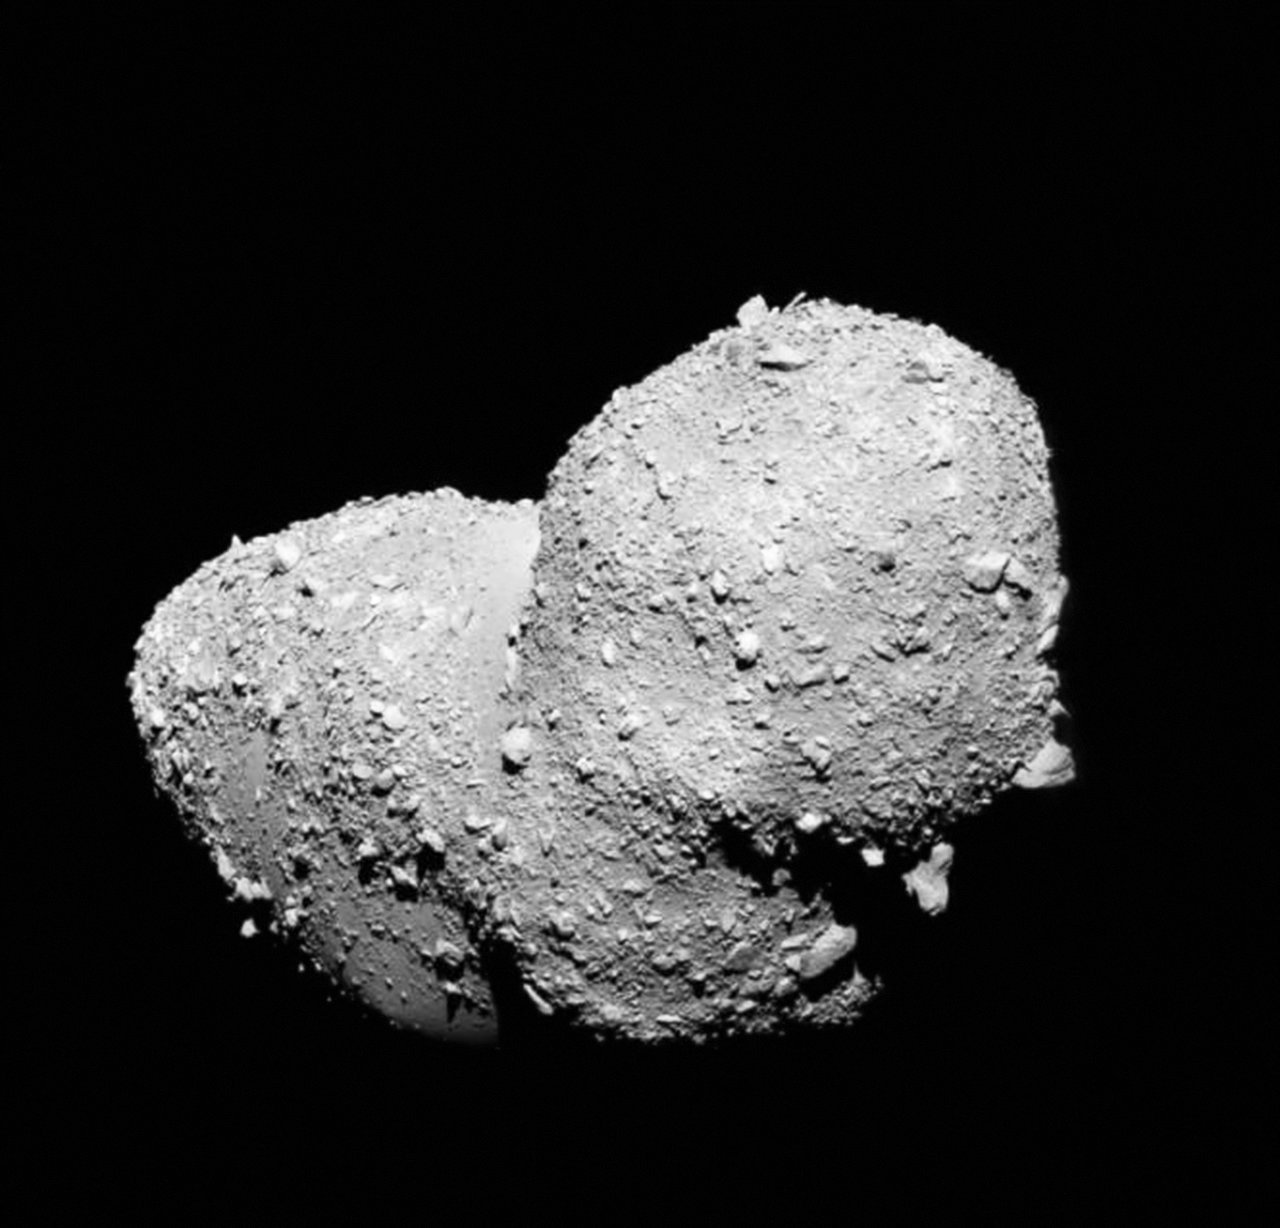
\includegraphics[height=0.3\textheight,width=0.5\textwidth, keepaspectratio]{figures/mathematical_background/eso1405b.jpg}}~
    \subcaptionbox{Comet 67/Churyumov-Gerasimenko\label{fig:67p}}{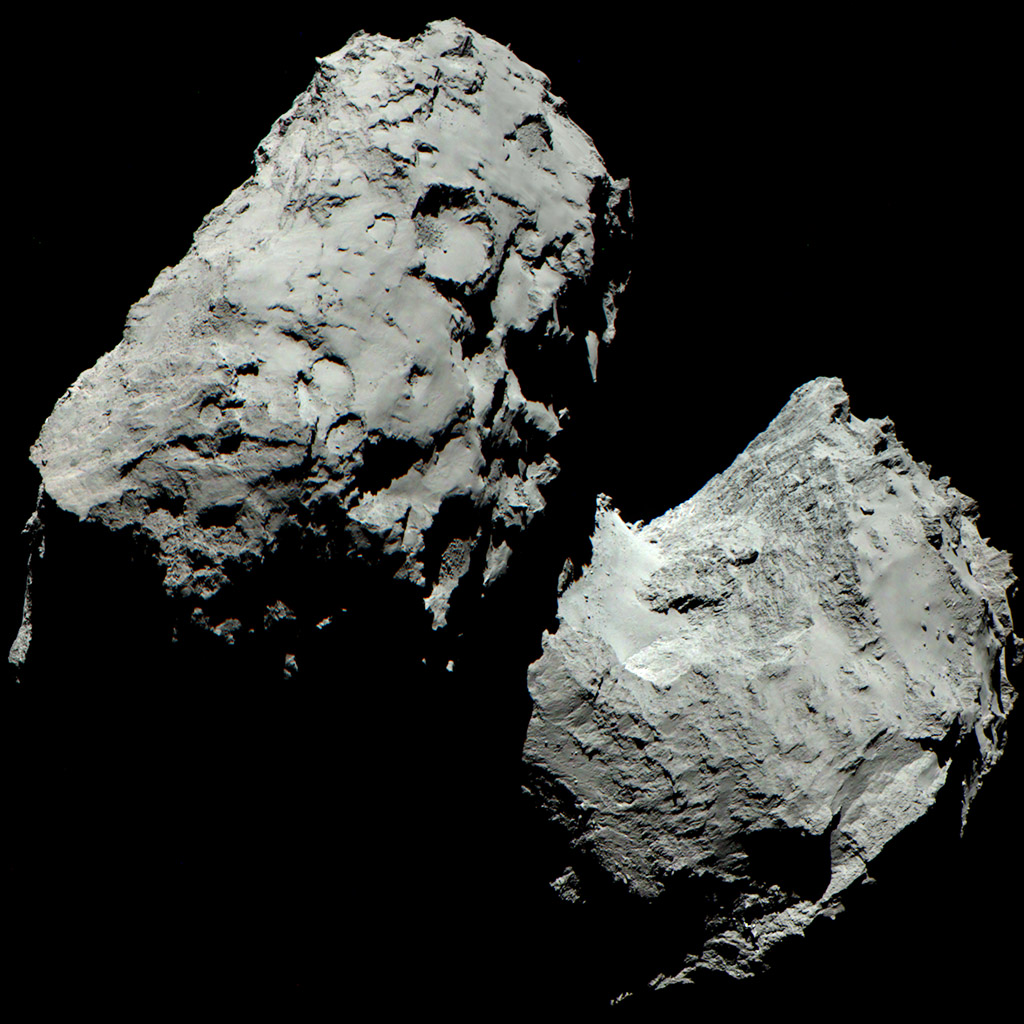
\includegraphics[height=0.3\textheight,width=0.5\textwidth,keepaspectratio]{figures/mathematical_background/comet67pcgin.jpg}}
    \caption{Examples of the non-ellipsoidal shapes of small solar system bodies. Both asteroids and comets will tend to have vastly irregular shapes due to their low mass and violent histories of impacts and collisions~\label{fig:irregular_asteroids}}
\end{figure}
The scientific community describes asteroid shape using the facet-vertex model.
This approach is an efficient representation of the more general notion of a polyhedron from geometry.
In this section, we define the notion of the polyhedron and some specifics of the format used in the astrodynamics community.

A polyhedron is a generalization of a two-dimensional polygon to three-dimensions~\cite{orourke1998}.
It is the region of space with a boundary defined by a surface of a finite number of polygonal faces.
The surface of the polyhedron is composed of three types of primitive objects: zero-dimensional points called vertices, one-dimensional segments called edges, and two-dimensional polygons called faces or facets.
Furthemore, without any loss of generality we assume each face is a convex polygon since any nonconvex face can be divided into smaller convex faces.
A valid polyhedron, in the context of asteroid shape models, must satisfy several constraints.
These constraints define the relationship between each of the types of primitives which make up the polyhedron surface.
The primitives must intersect ``properly'' and the local and global topology must be ``proper''.
For asteroid shape model we further assume that each face is a triangular polygon. 
Again, this does not limit generality as any polygon can be divided into a series of planar triangles.

The intersection of each face must be one of the following:
\begin{itemize}
    \item the faces are disjoint and do not intersect, or
    \item the faces meet at a single vertex, or
    \item the faces share two vertices and a common edge.
\end{itemize}
These intersection constraints automatically ensures that all edgeds and vertices intersect properly.
For example, edges that do not extend across an entire face or faces with penetrate would be improper and invalid.

The second constraint is related to the local topology around each point on the surface of the polyhedron.
In order to be locally proper, the neighborhood about any point on the surface of the polyhedron should be homeomorphic to a two-dimensional disk.
A neighborhood about any point on the surface is defined as an arbitrarily small subset or region of the surface which surrounds the point.
Every point on the surface should have a neighborhood which is topologically equivalent to a two dimensional disk.
The notion of equivalency is mathematically captured using the property of homeomorphism.
A homemorphism between two regions is a continous stretching or bending, without tearing or cutting, from one shape to another.
For example, it is possible to turn a circle into a square by a continuous stretching and bending of the shape.
However, it is not possible to transform a sphere into a torus, as this would require a hole to be created in the surface of the sphere.
The neighborhood about any point on the surface of the polyhedron should be equivalent to that of a two-dimensional disk.
A surface where this true for all points is called a \textit{two-manifold}, of a which the surface of a polyhedron is a subset.

The final constraint is related to the global structure of the surface in contrast to the local neighborhood of a point.
The surface must be connected, closed, and bounded.
In this sense, a connected surface is one where it is possible to travel from one point to any other point of the surface without leaving the surface. 
As a result, this will rule out any shapes with non-connected faces, such as a cube with a hollow interior/surface.
For example, on the outer surface of the cube it is not possible to reach a point on the interior surface. 
Combined with an assumption that there are a finite number of faces automatically ensures a closed and bounded surface. 
Note that these conditions do not in general rule out the possibility of holes passing completely through the object.
For example, a torus, or a donute shape, is also considered a polyhedron.
The key difference between a hole and a cavity is that there are no disconnected surfaces and as a result a polyhedron can have any number of such holes. 
In practice, we tend to limit our analysis to polyhedron with no holes, or with a genus of zero.

\subsection{Polyhedron Data Structure}
While the shape of the asteroid will be represented mathematically as a polyhedron, we are still left with the issue of representing this shape in digital form. 
The eventual computational efficiency and memory consumption of the subesequent sections is heavily dependent on the underlying data structure used to represent the surface.
In this section, we review some of the basic requirements and features of any data structure.
In addition, we summarize the ones most popular in the astrodynamics community and the halfedge data structure which we use in this work.

The requirements for any surface/mesh data structure vary between applications and are designed to satisfy both topological and algorithmic requirements.
Some examples of topological considerations are the use of triangular/polygonal facets or the ability to represent manifold/non-manifold meshes.
Examples of algorithmic requirements include a consideration of the types of algorithms/processes that will make use of the data, such as visualization or operations that will modify or additional data to the various faces, edges, and vertices of the mesh.
The choice, and eventual design, of an appropriate data structure is evaluated on its ability to efficiently enable specific operations, such as distance or modification operations.
A wide variety of data structures have been developed to represent general polyhedron surfaces and can be classified as either \textit{face-based} or \textit{edge-based}.

The simplest method to represent a surface mesh is composed to storing the individual vertices which define each face of the surface.
In the specific case of a triangular mesh, this entails storing the three vertex coordinates of each face of the mesh, also called the \textit{face-set}~\cite{botsch2010}.
By assuming that the vertex coordinates are stored as double precision, or \SI{64}{\bit} values, results in \( 3 \cdot 3 \cdot 64 = \SI{576}{\bit} = \SI{72}{\byte}\) per triangular face.
% TODO Add reference to euler's formula
Equivalently, from Euler's formula, there is approximately twice as many faces as vertices, and this \textit{face-set} structure will require on average \SI{144}{\byte} per vertex.
A simple optimization is possible by reducing the redundancy in the representation.
Each vertex will duplicated as many times as the degree of the vertex.
This redundancy can be eliminated by storing a list of vertices, and to define the vertices of each face as an index/reference into this vertex list.
This results in the so called \textit{indexed face set} or \textit{shared-vertex} data structure.
In the case of triangular meshes and using double precision values, each vertex will require \(\SI{192}{\bit} = \SI{24}{\byte}\).
Vertex indices of each face can be stored using single precision, \( \SI{32}{\bit} = \SI{4}{\byte}\), values which resuts in a storage requirement of \( \SI{96}{\bit} = \SI{12}{\byte}\) per triangle.
This type of representation will therefore require on average approximately \( \SI{60}{\byte} \) per vertex, which is half the requirement of the \textit{face-set} data structure.
\begin{figure}
    \centering
    \includegraphics[width=\textwidth]{example-image-golden}
    \caption{Face based data structure look in PMP Fig2.3 or 2.4~\label{fig:face_based_data_structure}}
\end{figure}
% TODO add acronyms/glossary items for these terms
Examples of this type of data structure include the stereolithography (STL), Wavefront (OBJ), OFF, and VRML file formats.

While conceptually simple the face based data structure has several critical drawbacks.
It is difficult to determine the connectivity of individual vertices or faces of the mesh, which makes it ill-suited for most algorithms.
The vast of majority of computational geometry algorithms will require as a minimum~\cite{botsch2010}:
\begin{itemize}
    \item Access to individual vertices, edges and faces, as well as random access to any element.
    \item Enumeration of the edges of a single face.
    \item Access to the adjacent faces of an edge which enables access to the neighboring faces.
    \item Given an edge one must determine the two vertices which define the endpoints.
    \item Given a vertex one must determine all neighboring faces.
\end{itemize}
As a result, any application making use a face based data structure will need to store additional connectivity information in a seperate data structure.

In contrast to face-based structures, edge-based data structures store the connectivity information in the edges or halfedges~\cite{botsch2010,orourke1998}.
By splitting each unorientated edge into two orientated halfedges, the halfedge data structure provides an efficient data structure for mesh based operations.
Each halfedge is ordered in a clockwise fashion around each face, typically such that the face normal is orientated outwards from the mesh.
In addition, each halfedge will also store a reference to:
\begin{itemize}
    \item The vertex it points to, or its target,
    \item its adjacent face,
    \item the next halfedge of the face in a counterclock wise direction,
    \item the previous halfedge of the face
    \item the opposite or incident halfedge.
\end{itemize}
In addition, each face stores the reference to one of its halfedges, while each vertex stores an outgoing halfedge. 
The halfedge data structure will require more memory in contrast to face based approaches it offers several advantages which make it ideal for computational geometry operations.

A halfedge data structure allows us to iterate through all elements, vertices, edge, halfedge, or face, in a simple manner.
In addition, the halfge edge data structure can store arbitrary polygon meshes.
Furthermore, additional data can be attached to the elements as each is store explicitly.
Finally, the halfedge data structure allows for simple manipulation and modification of the underlying mesh, enabling operations such as mesh subdivision or simplification.
There are a number of publicly avaiable implementations of the halfedge data structure~\cite{cgalproject2018,botsch2002}.
We utilize the \texttt{Surface\_mesh} data structure implemented within the Computational Geometry Algorithms Library~\cite{sieger2011}.
This provides a well defined and highly optimzed data structure for the representation of the polyhedron shape of the asteroid.
Furthermore, the ability to incorporate additional properties enables us to efficently compute the polyheron potential model.
\begin{figure}
    \centering
    \includegraphics[width=\textwidth]{example-image-golden}
    \caption{Halfedge data structure look in PMP Fig3.4~\label{fig:halfedge_data_structure}}
\end{figure}

\begin{figure}
    \centering
    \includegraphics[width=\textwidth]{example-image-golden}
    \caption{Iterating over 1 ring of a vertex}
\end{figure}

\subsubsection{Wavefront OBJ files}
The OBJ format is a geometry definition file format used for a variety of computer modeling applications, and is regularly used by the asteroid community~\cite{neese2004}.
The basic format of the file is an ASCII file where the first \( N_v\) lines begin with \texttt{v} and define the three components of a vertex in the body fixed reference frame.
The following \( N_f\) lines begin with \texttt{f} and define the three indices of the vertices that make up the face.
The numbering of the vertices is implicitly defined by the order listed in the file, i.e. the vertices are defined from \( 1 \) to \( N_v\).
There are two main assumptions used by the asteroid community.
First, each face is triangular and second, the vertices are numbered in a counterclockwise fashion about each face.
This allows the outward facing normal to each face to be uniquely defined without any additional data.

This polyhedron model, captured using the OBJ format, allows for a much larger class of potential object shapes. 
The accuracy of the shape model can be arbitrarily improved by incorporating additional vertices and faces, which increase the resolution of the model in regions of high complexity.
The polyhedron model can capture arbitrary depressions, ridges, or holes through the asteroid.
Small bodies typically lack sufficient mass to create regular, spherical shapes, and exhibit a large variety in resulting shapes such as the examples shown in~\cref{fig:asteroid_shape}.
\begin{figure}
    \centering
    \subcaptionbox{4769 Castalia\label{fig:castalia}}{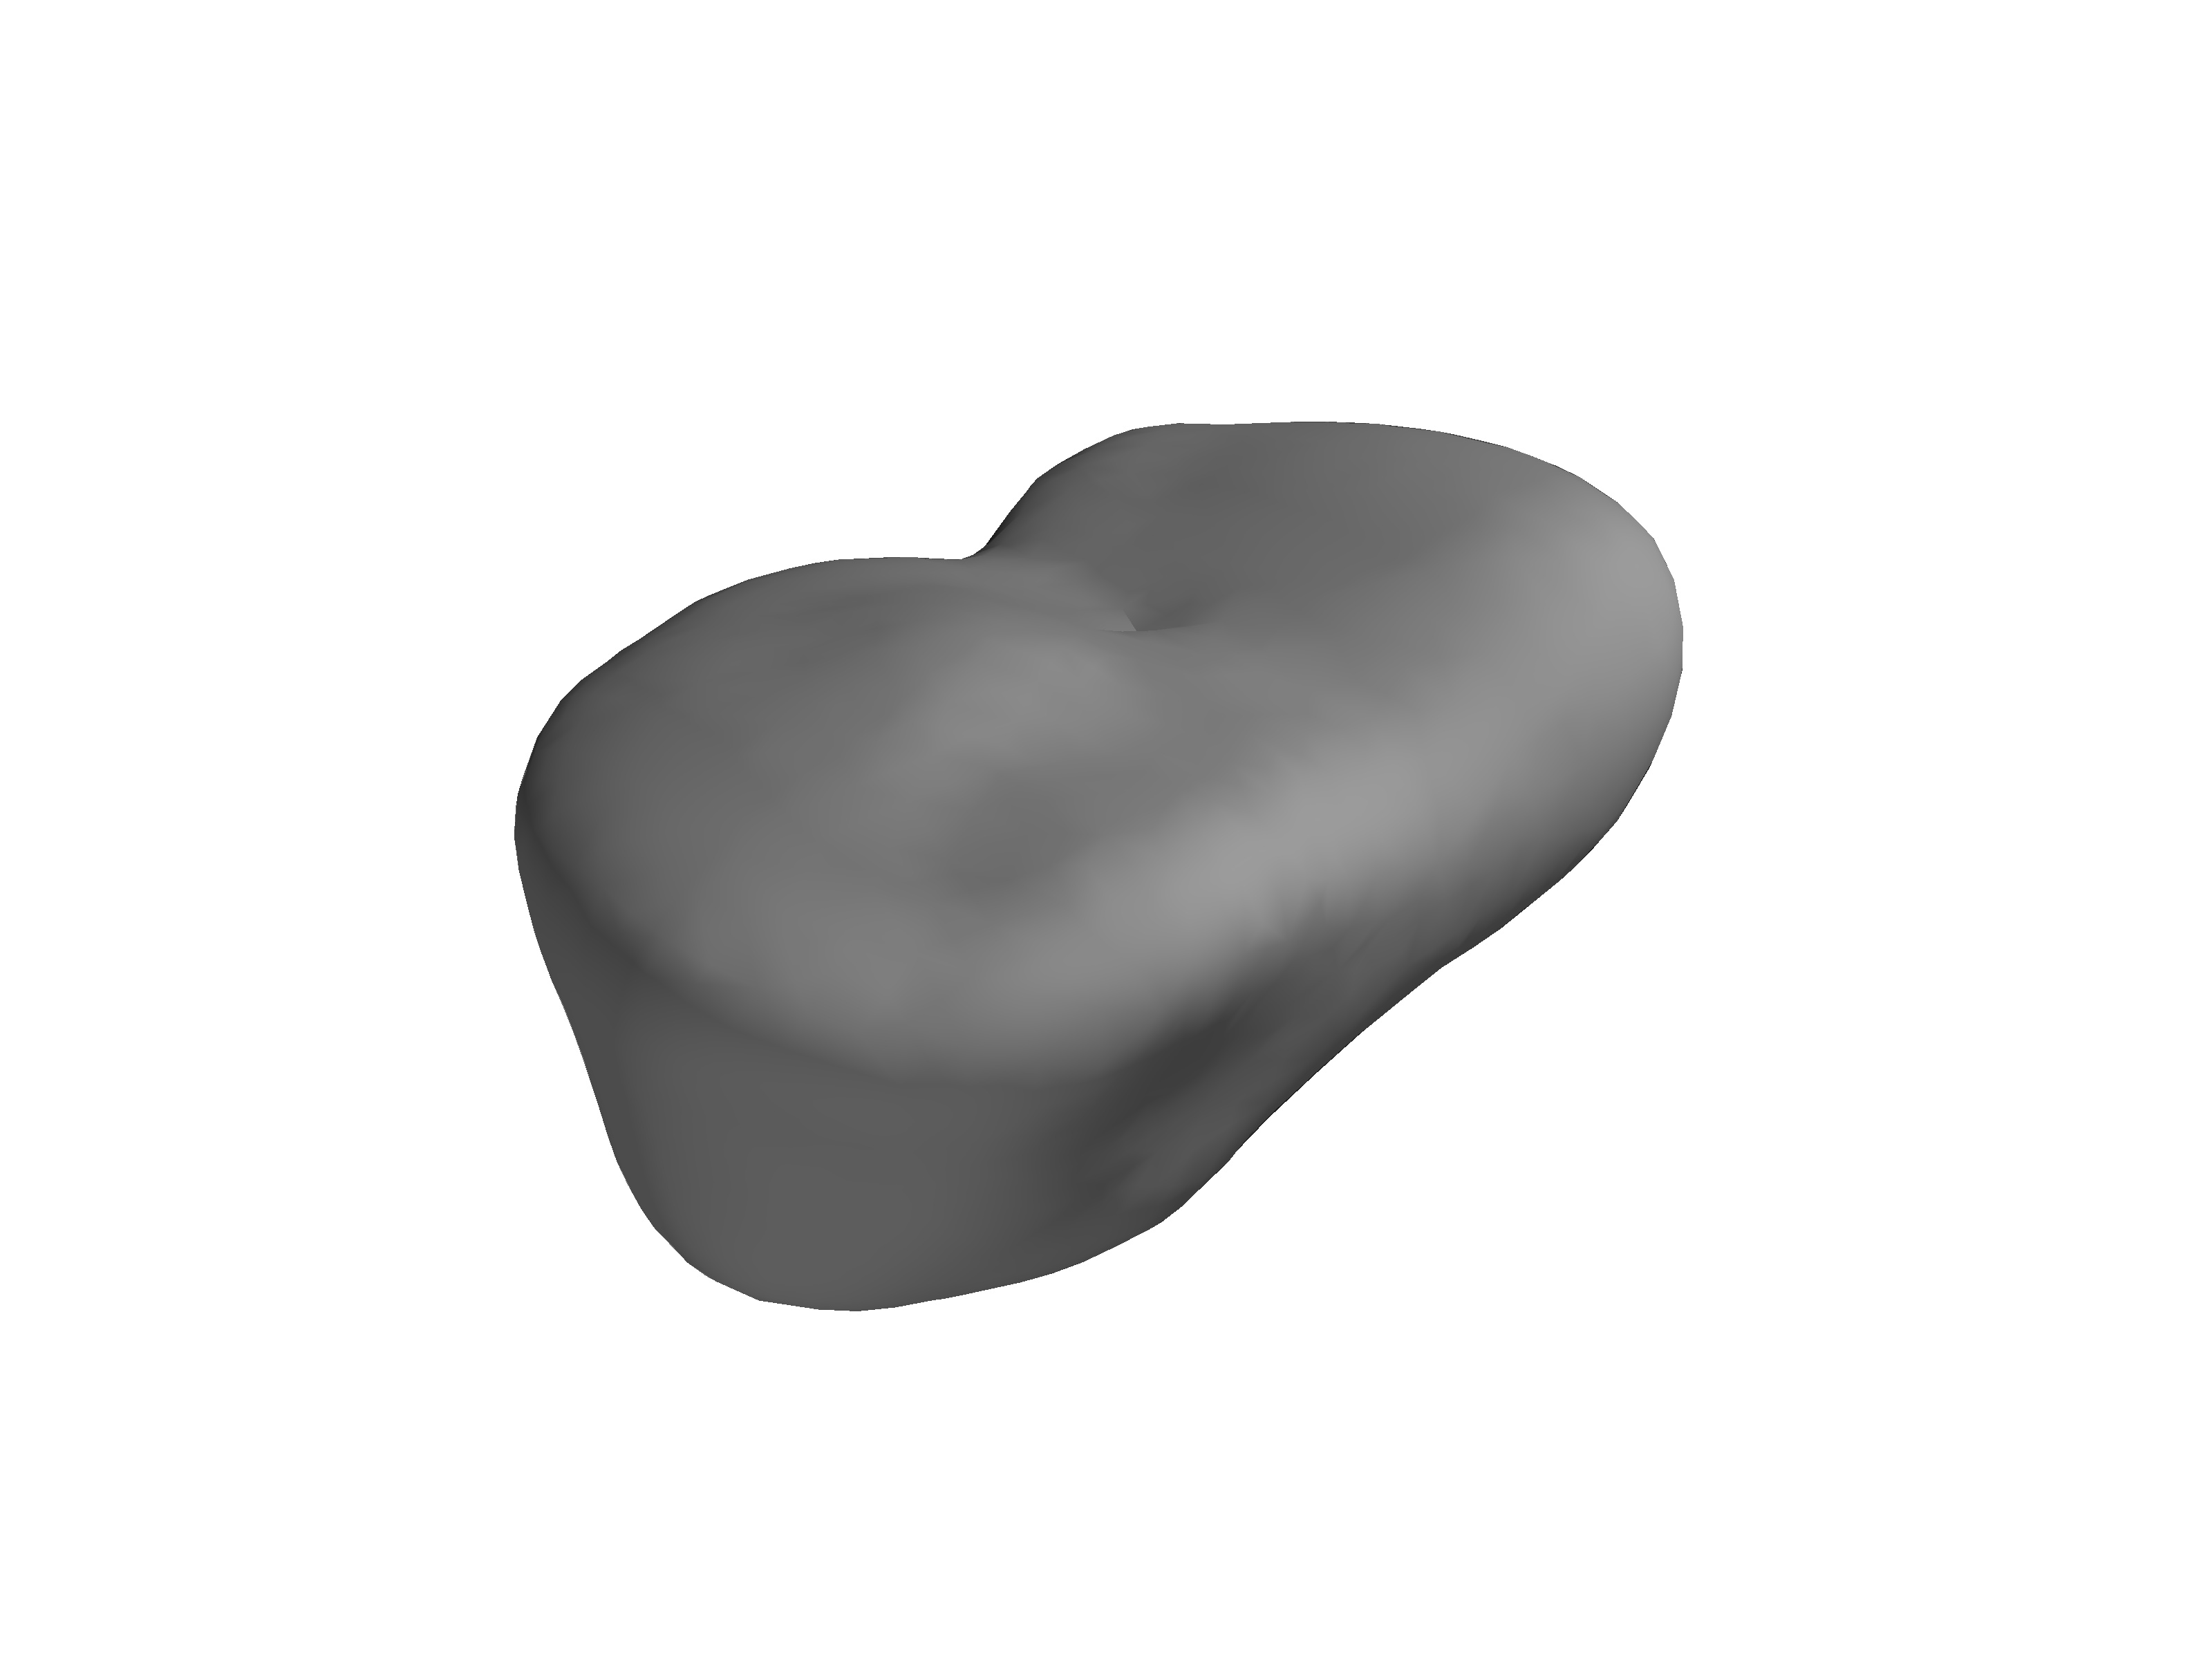
\includegraphics[width=0.33\textwidth]{figures/mathematical_background/castalia_isometric.jpg}}~
    \subcaptionbox{Geographus\label{fig:geographus}}{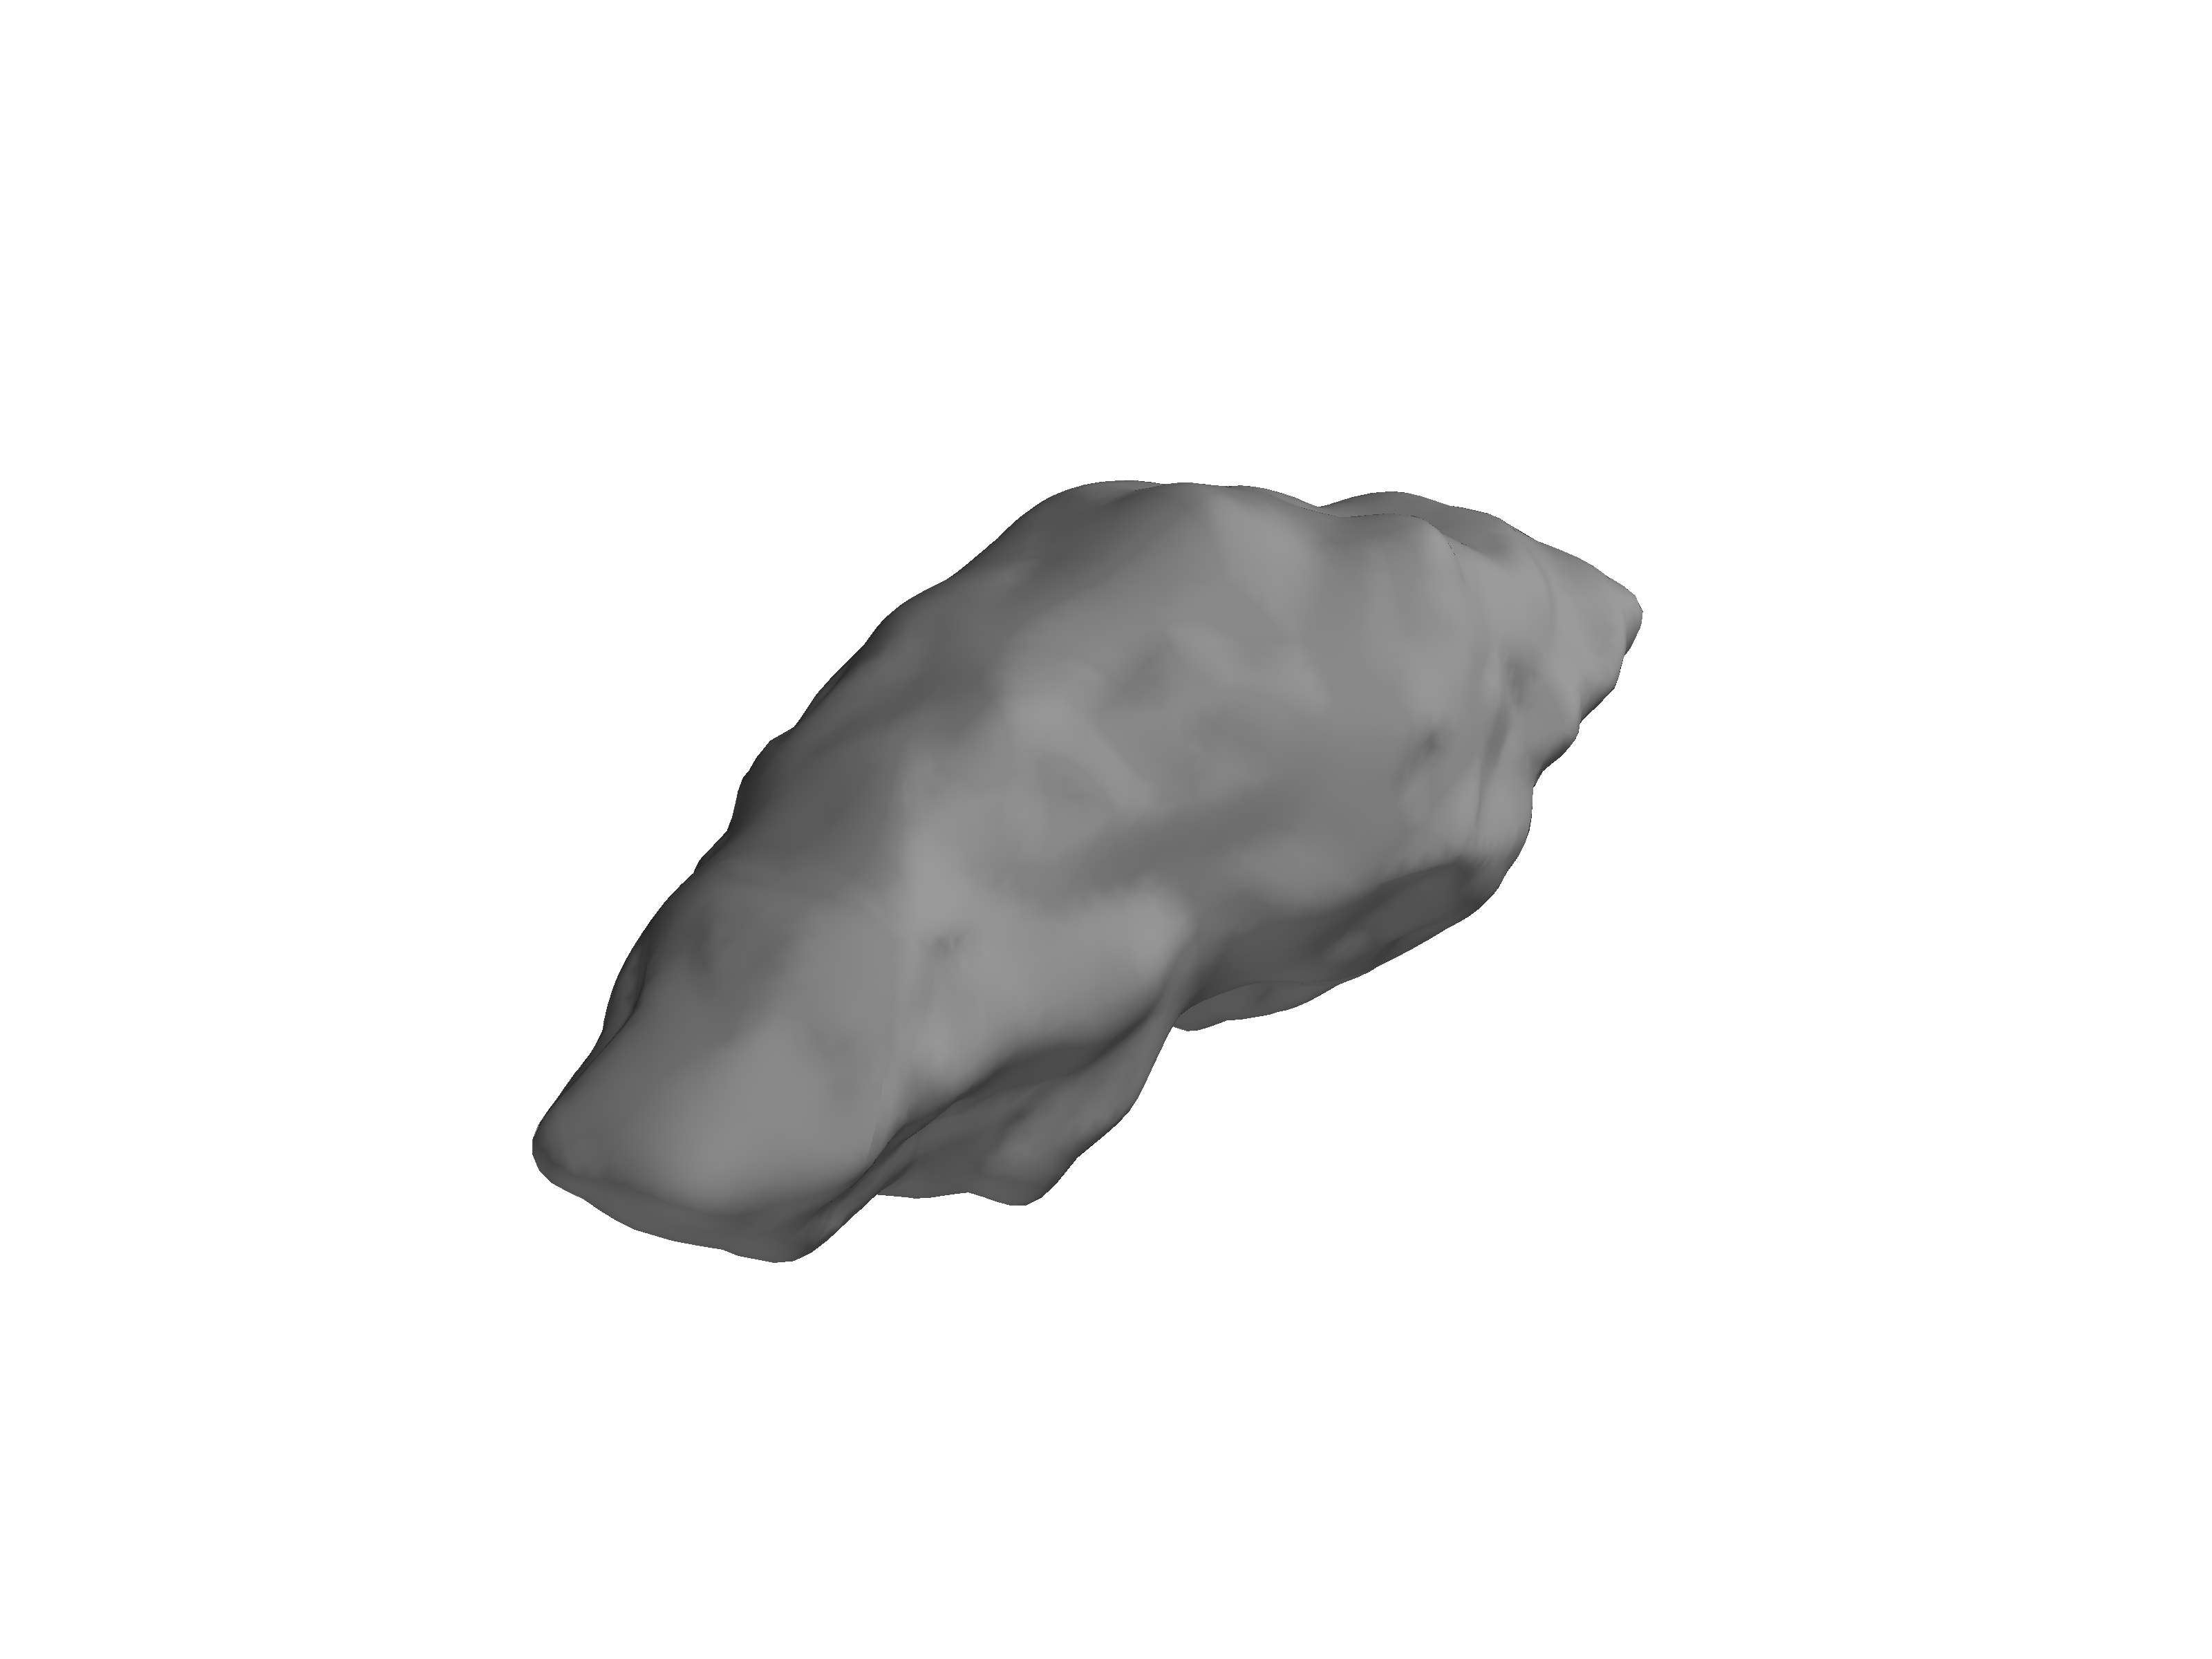
\includegraphics[width=0.33\textwidth]{figures/mathematical_background/geographus_isometric.jpg}}~
    \subcaptionbox{Golevka\label{fig:golevka}}{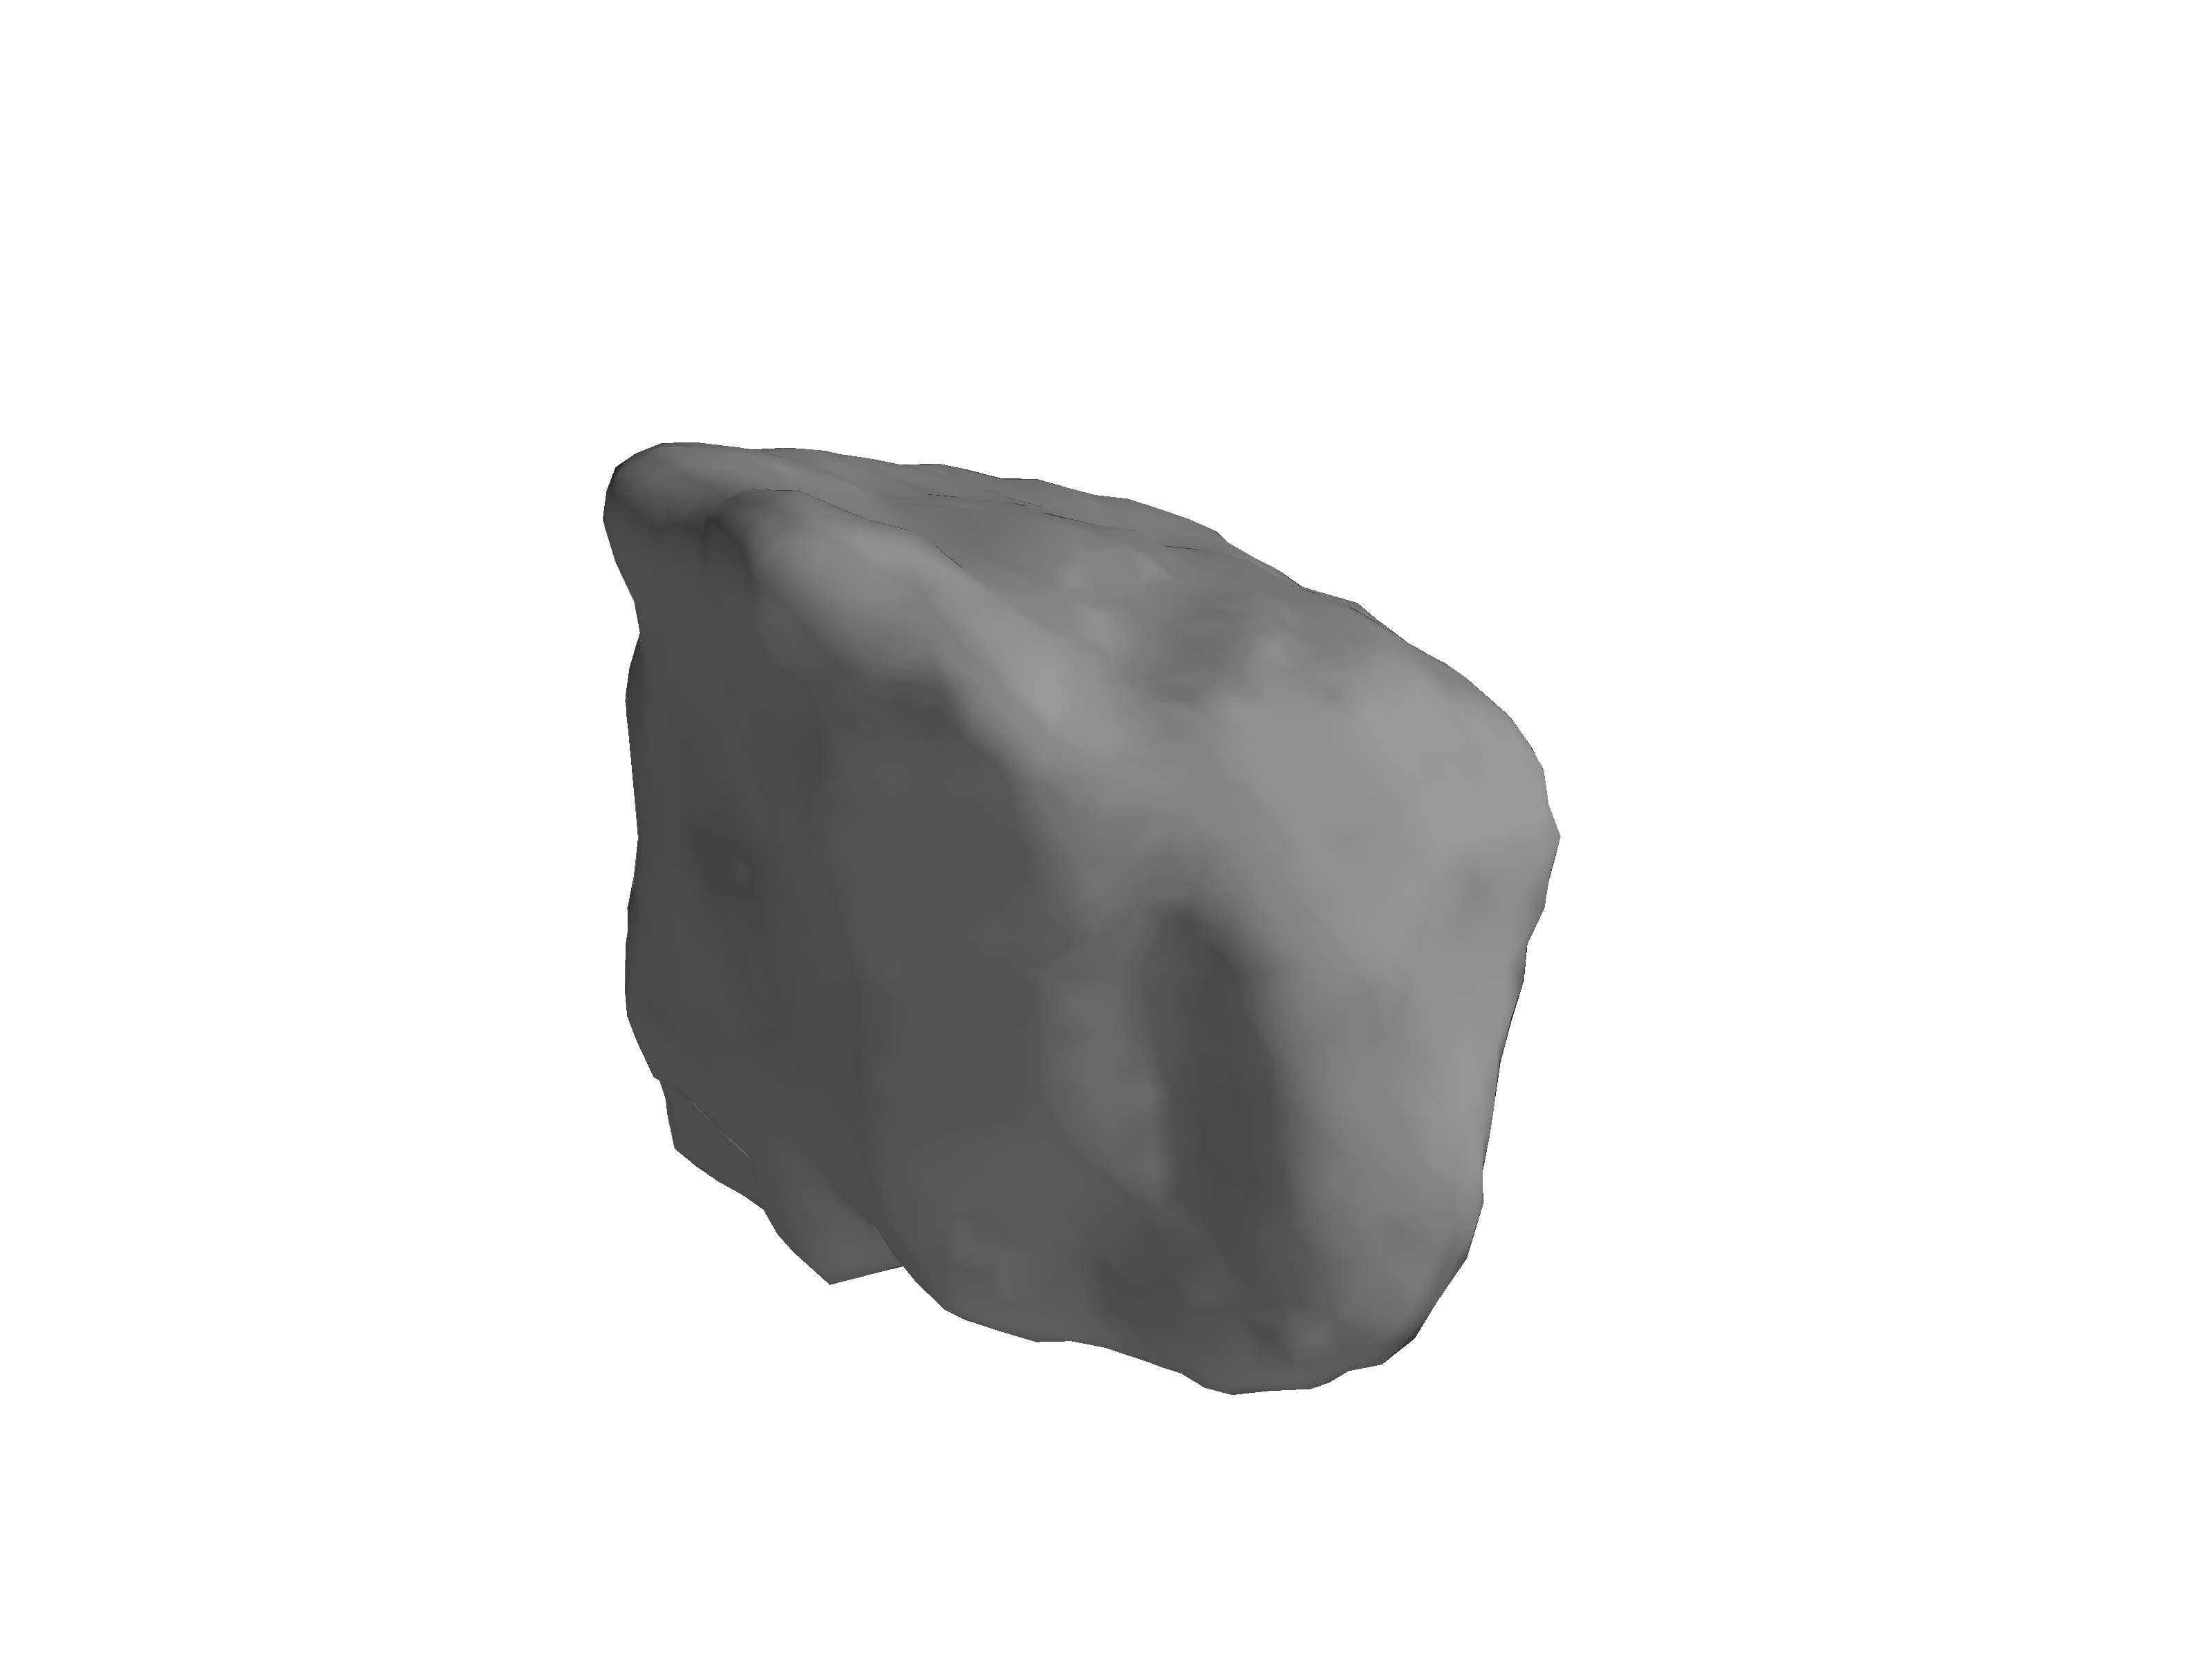
\includegraphics[width=0.33\textwidth]{figures/mathematical_background/golevka_isometric.jpg}}
    \caption{Polyhedron Shape Models for several asteroids~\label{fig:asteroid_shape}}
\end{figure}
Polyhedron shape models are available for several asteroids~\cite{neese2004,gaskell2008b}.
The quality and resolution is dependent on the measurement available of the body.
\Cref{fig:itokawa_radar} shows a polyhedron model of asteroid 25143 Itokawa based on ground radar measurements~\cite{neese2004}.
This model is composed of \num{6098} vertices and \num{12192} faces and captures the general ellipsoidal shape of the asteroid.
However, ground based measurements are unable to provide the resolution required to capture the fine details or even the asymmetry of asteroid Itokawa.
In contrast,~\cref{fig:itokawa_insitu} shows the model derived from in-situ measurements from optical sensor of the Hyabusa spacecraft~\cite{gaskell2008a}.
It is composed of \num{1579014} vertices and \num{3145728} faces and is able to capture small surface features such as boulders.
\begin{figure}
    \centering
    \subcaptionbox{25143 Itokawa Radar Model\label{fig:itokawa_radar}}{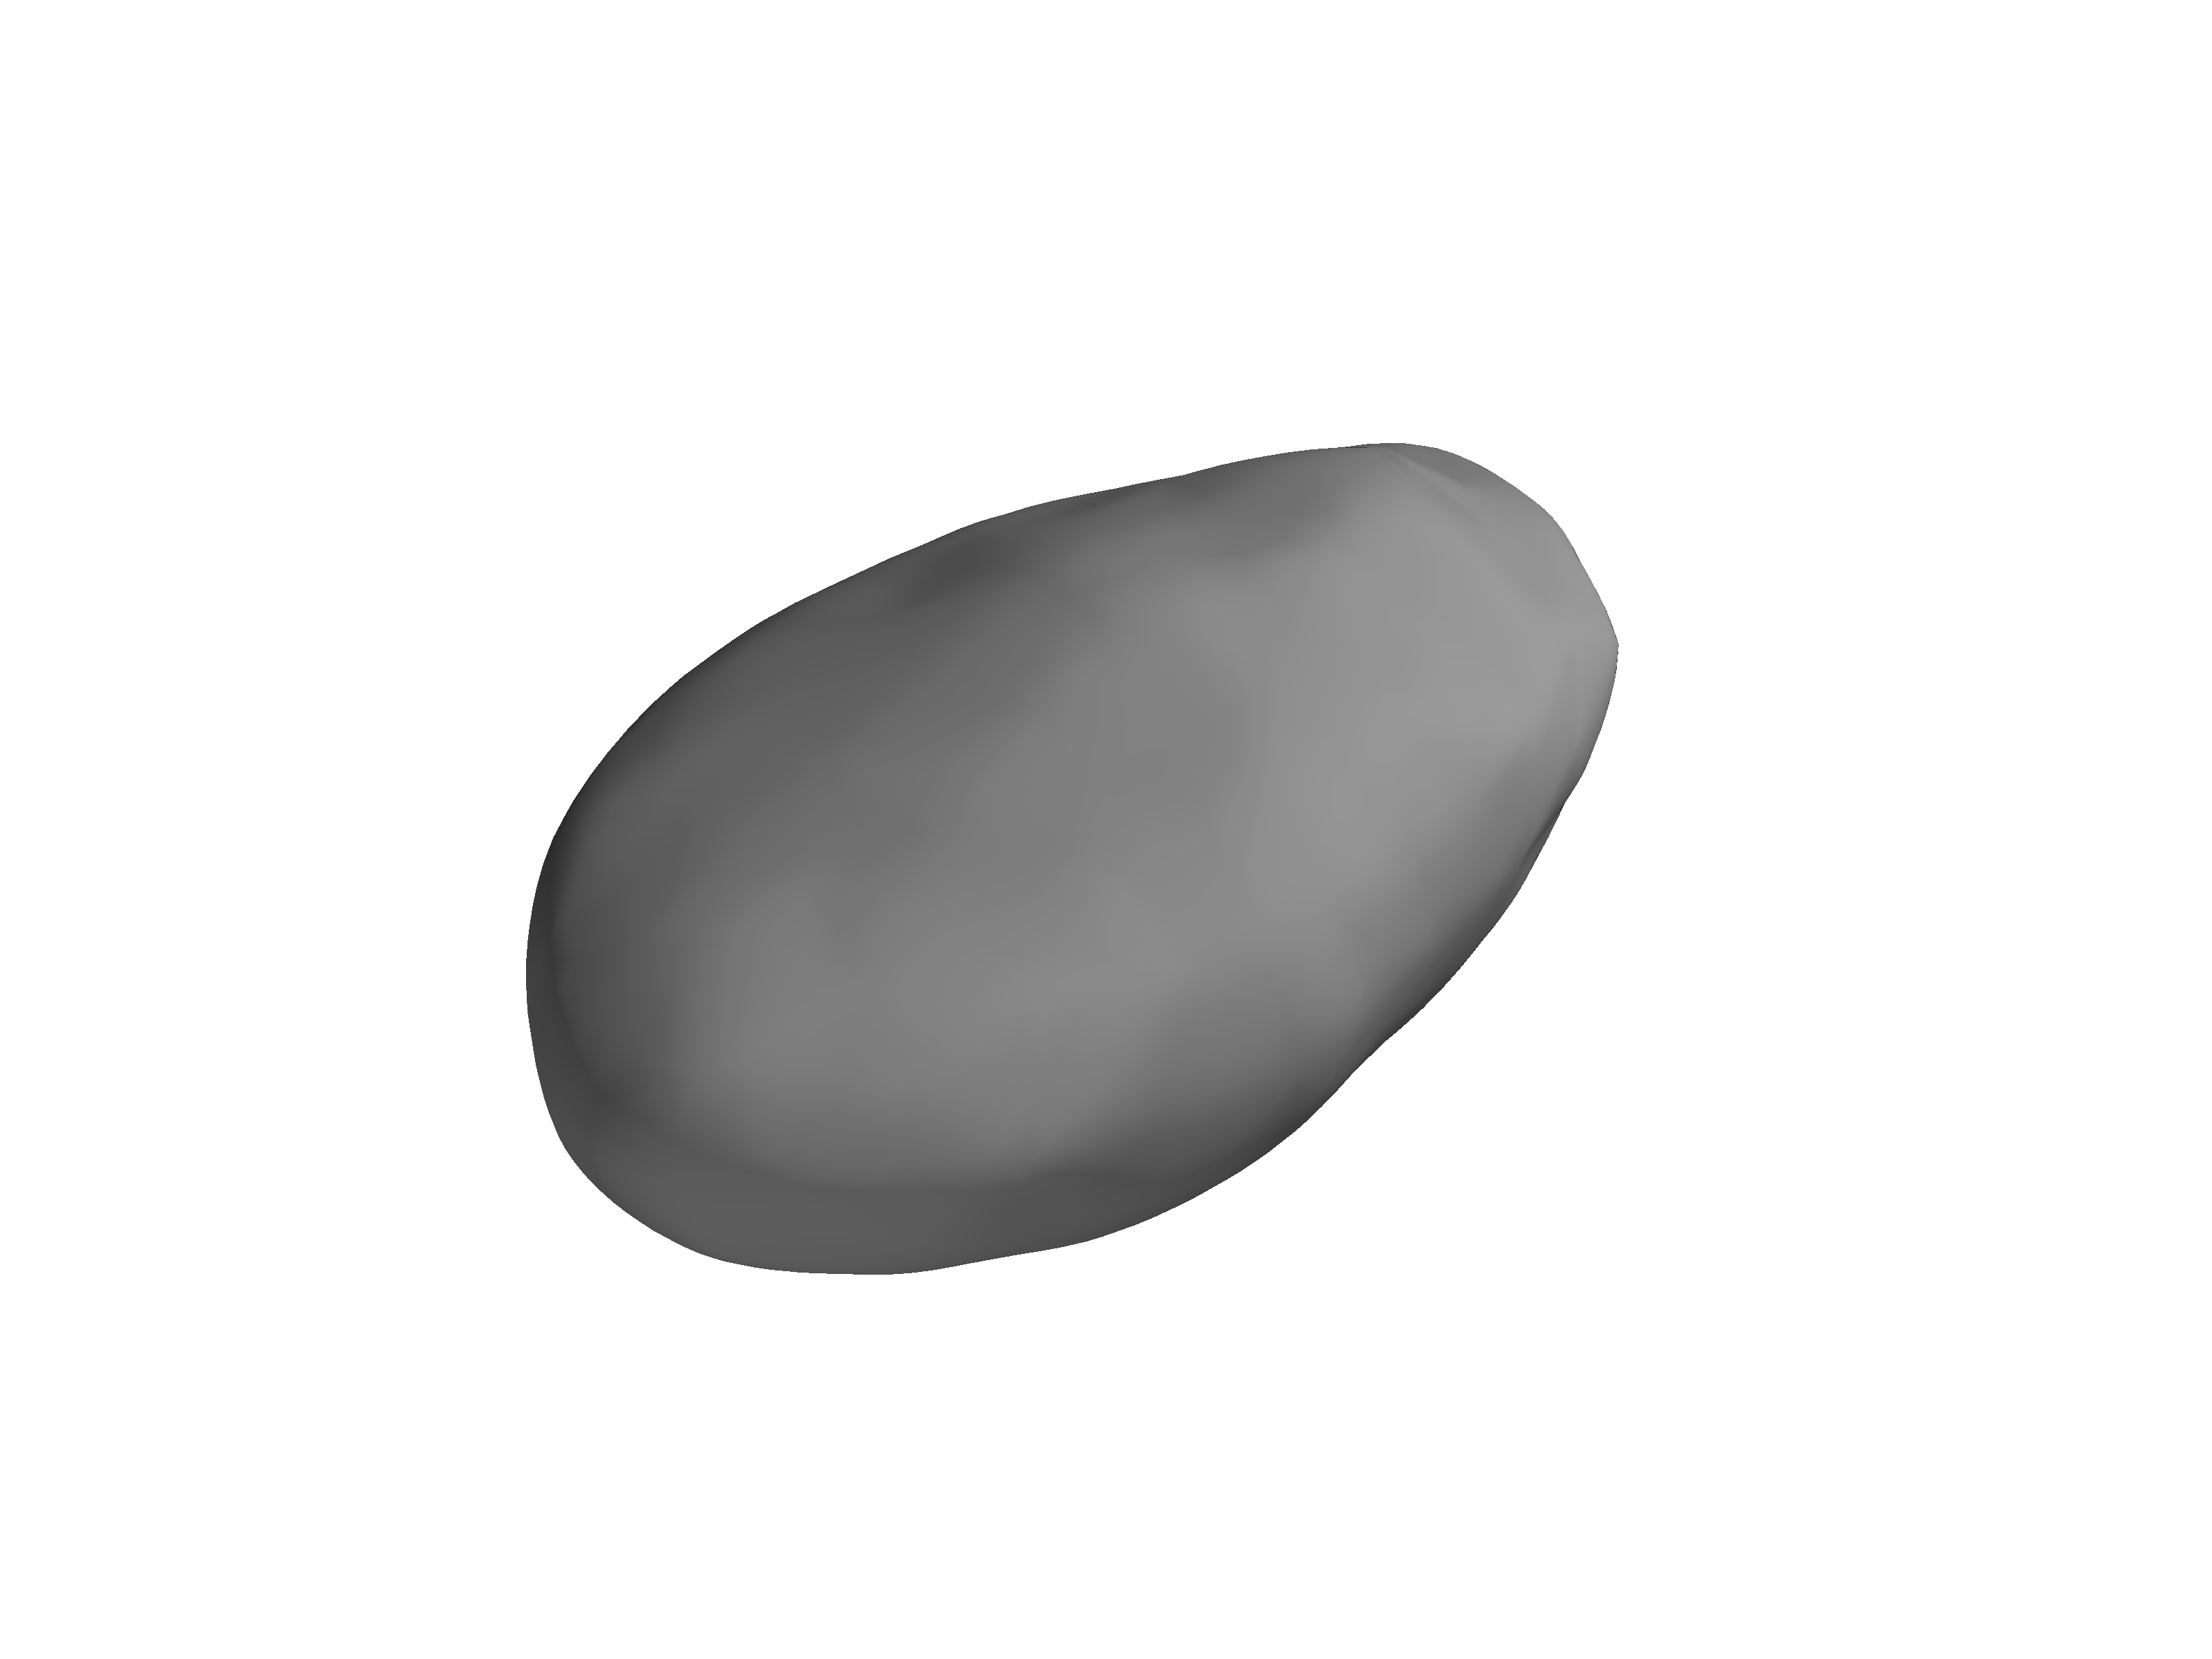
\includegraphics[width=0.5\textwidth]{figures/mathematical_background/itokawa_radar_isometric.jpg}}~
    \subcaptionbox{25143 Itokawa In-Situ Model\label{fig:itokawa_insitu}}{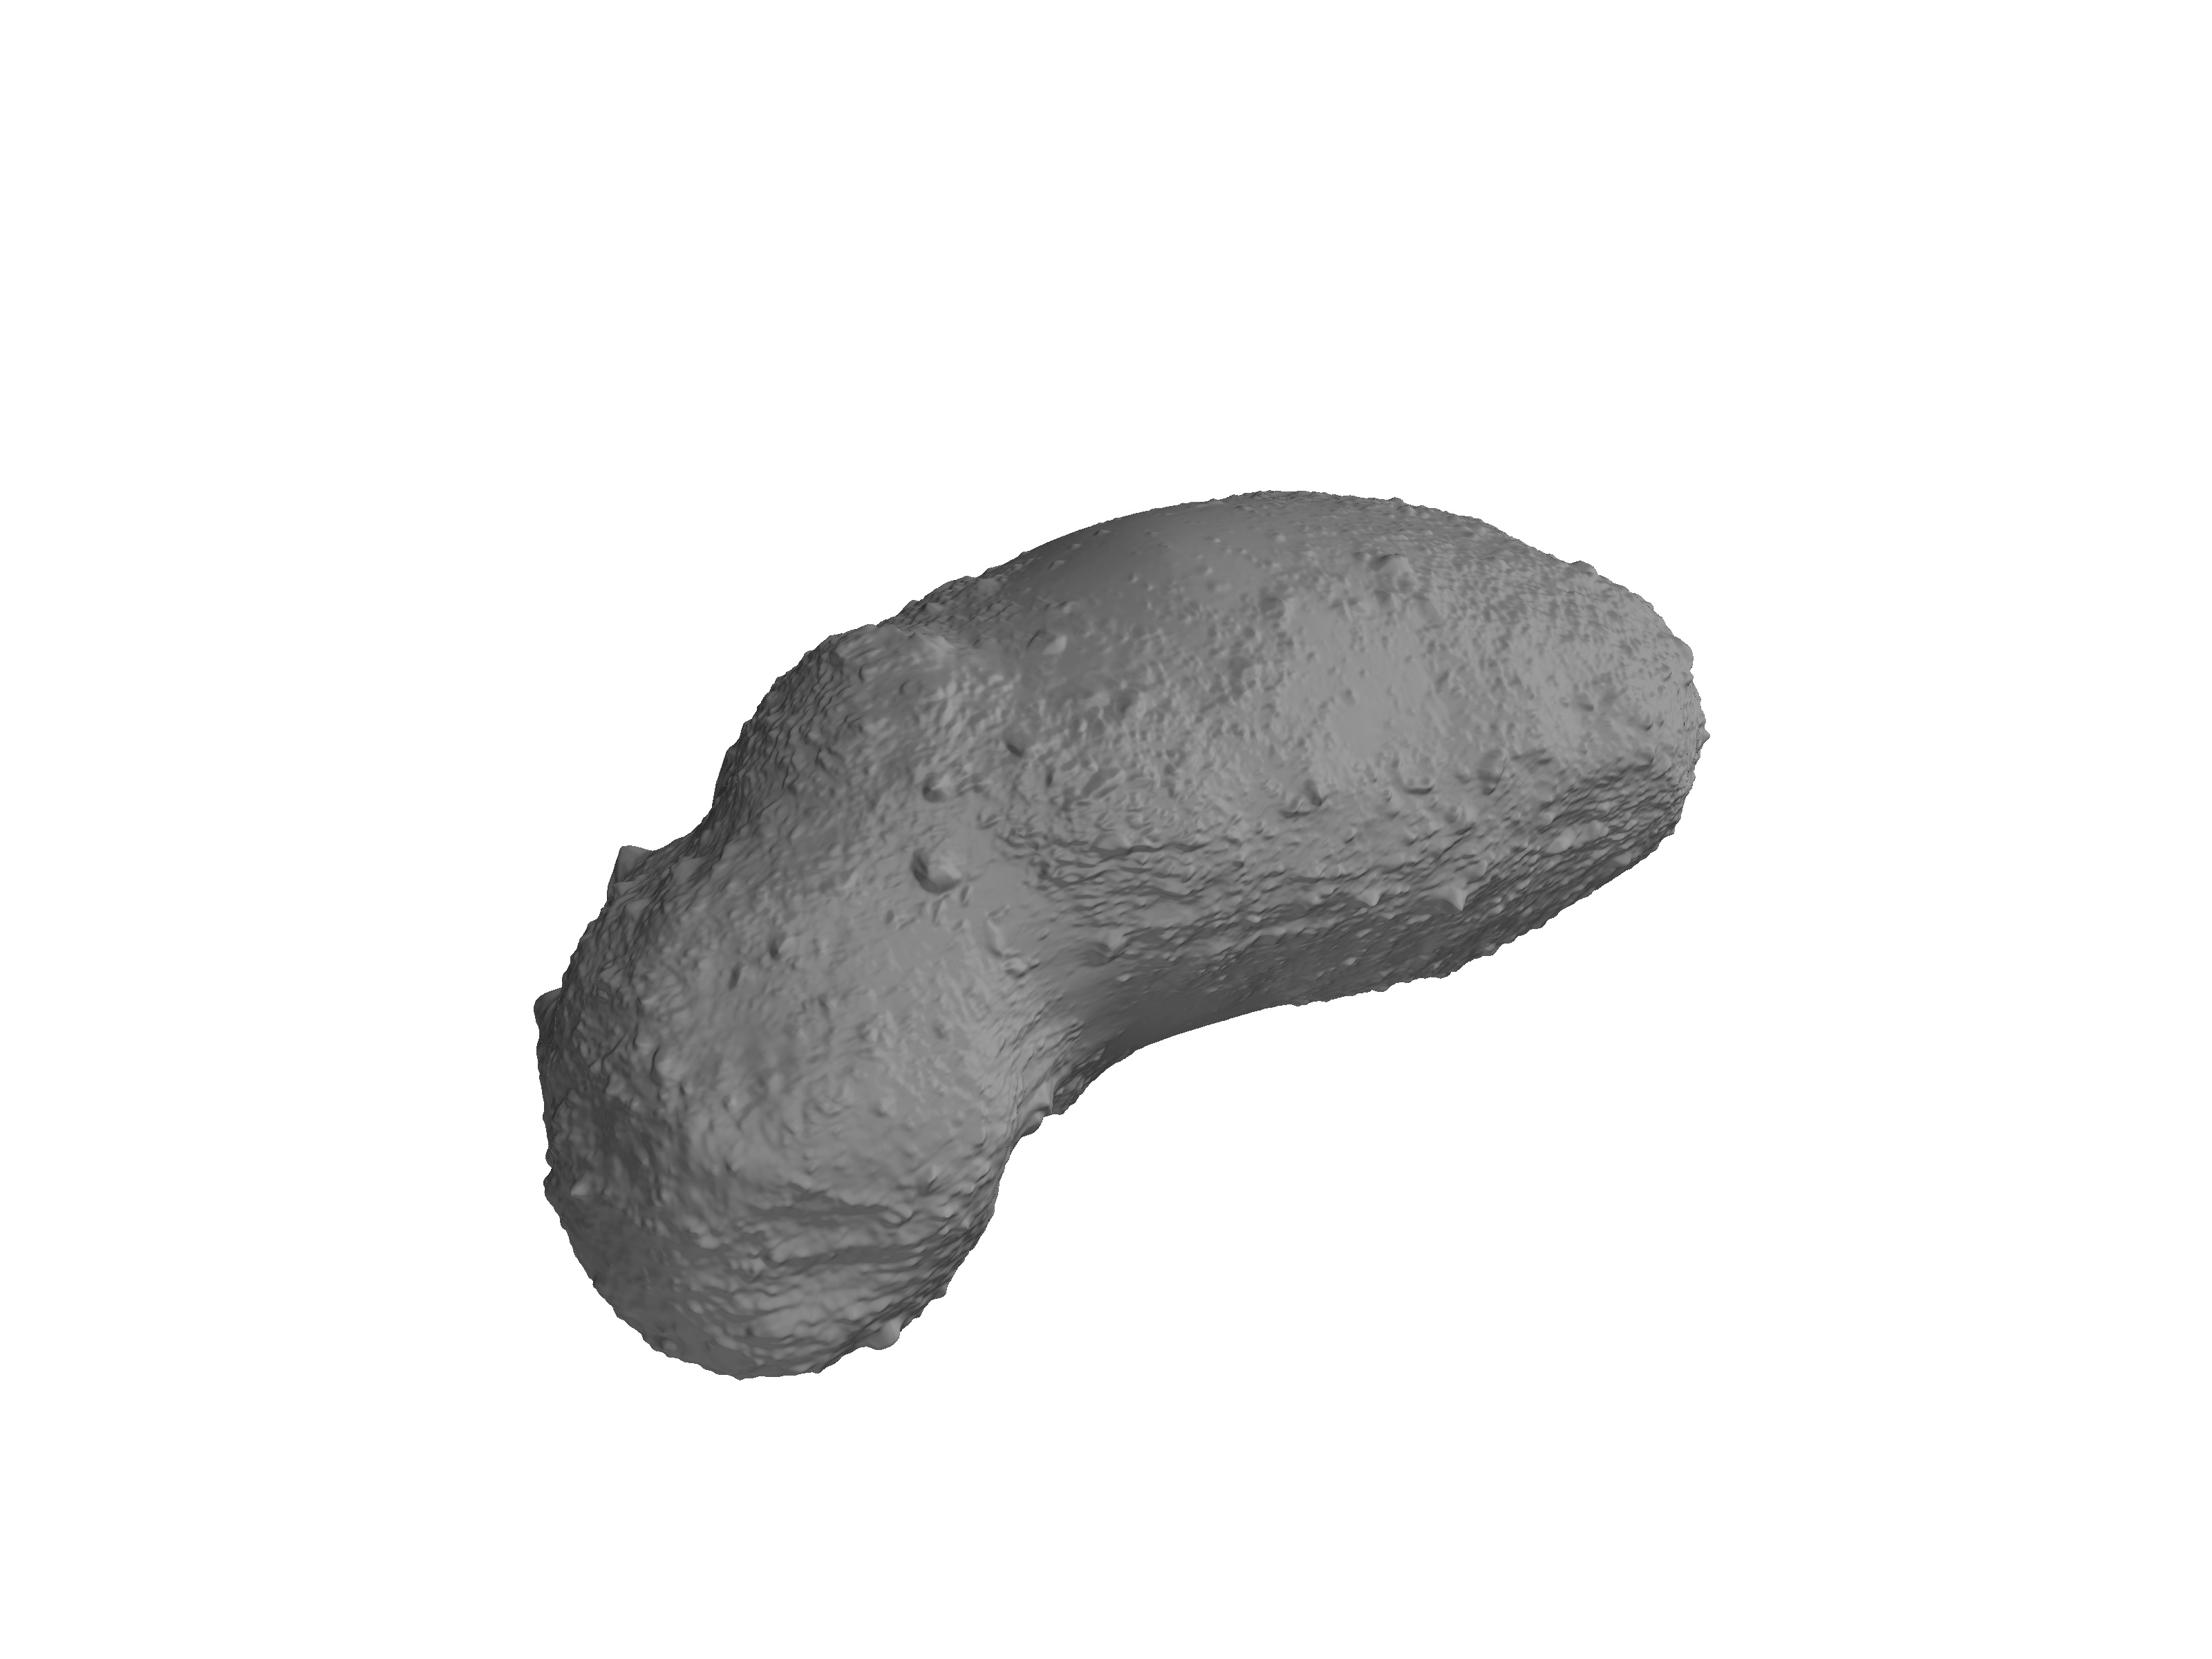
\includegraphics[width=0.5\textwidth]{figures/mathematical_background/itokawa_isometric.jpg}}
    \caption[Comparison of Radar and In-situ Itokawa models]{Comparision of polyhedron models of 25143 Itokawa based on ground based radar or in-situ measurements.
        The ground based model can capture the rough ellipsoidal shape but does not capture fine surface details.}
\end{figure}
From this simple example, it is clear that prior to the arrival of a spacecraft the shape and surface knowledge of an asteroid is limited.

\section{Gravitational Models around Small-Bodies}
Due to the irregular shape of small-bodies, the gravitational field around these bodies is equally irregular.
Furthermore, the relative size of the spacecraft in comparison with the orbital radius and small-body creates a much larger coupling between the translational and rotational states of the spacecraft.
In addition, spacecraft will tend to operate in very close proximity to the surface.
As a result, accurate computation of the gravitational field around these irregular bodies is critical to safe and effective operations.
The classic approach to determining the gravitational force is to apply Newton's law of Universal gravitation.
The force due to gravity between two point masses is defined as
\begin{align}\label{eq:newton_universal_gravitation}
    \vb{F}_g =  - G \frac{m_1 m_2}{r^2} \frac{\vb{r}}{r},
\end{align}
where \( G \) is the universal gravitational constant, \( \vb{r} \) is the relative position vector between the points of mass \( m_1, m_2\), respectively.

\begin{figure}
    \centering
    \includegraphics[width=\textwidth]{example-image-golden}
    \caption{Newton's Law of Unviversal Gravitation~\label{fig:universal_gravity}}
\end{figure}

This gravitational model is defined if point masses or bodies which can be modeled as point masses, such as spherically symmetric planets.
However, it is not possible to model an irregular asteroid, or an orbiting spacecraft, as point masses.
Instead, one must treat both bodies as extended objects and compute the gravitational force from the potential function as an integral over the entire body
\begin{align}\label{eq:volume_integral_potential}
    \vb{F}_g = \nabla U = G \int_V \frac{1}{r} dm,
\end{align}
where \( r = \norm{\vb{r}} \) and \( \nabla U \) is defined as the gradient of \( U \) with respect to the standard cartesian basis vectors
\begin{align*}
    \nabla = \deriv{}{x} \hat{\vb{i}} + \deriv{}{y} \hat{\vb{j}} + \deriv{}{z} \hat{\vb{k}}.
\end{align*}
There are large variety of methods to evaluate the volume integral in~\cref{eq:volume_integral_potential}.

The first approach, sometimes termed the \textit{mass-concentration}, or \textit{mascon} method, approximates the integral using an infinite sum of point masses \( m_i\) located at \( \vb{r}_i \).
The potential on our object of interest then becomes the summation of the potential caused by each mass \( m_i \) as shown in~\cref{eq:mass_con_potential}.
\begin{align}\label{eq:mass_con_potential}
    U = G \sum_{i=0}^{\infty} \frac{m_i}{\norm{\vb{r} - \vb{r}_i}}
\end{align}
The method distributes a colleciton of point masses uniformly throughout the body such that the total mass is equal to the body.
While conceptually simple, and relatively straight forward to numerically implement, the mascon approach has several drawbacks~\cite{scheeres2012a}.
First, the mascon approach does not provide any method to determine if the object of interest is inside or outside of the body.
As a result, any numerical simulation making use of the mascon approach will require a secondary operation to determine if the spacecraft has collided with the surface.
Additionaly, it has been shown that the mascon approach is more computationaly demanding than other methods, namely the spherical harmonic or polyhedron potential method~\cite{werner1996}.
Finally, while the mascon method will provide the true gravity field in the limit as the number of invidual point masses becomes large, there are significant errors in the direction of the force vector~\cite{werner1996}.

It can be shown that the gravitational potential will satisfy Laplace's equation outside of the body
\begin{align}
    \nabla^2 U = 0
\end{align}
and Poisson's equation inside of the body
\begin{align}
    \nabla^2 U = - 4 \pi G \sigma
\end{align}
where \( \sigma \) is the local density of the body.
Laplace's equation can be solved using a seperation of variables in terms of spherical coordinates~\cite{scheeres2012a}.
The transformation between cartesian, \( \vb{r} = x \hat{\vb{x}} + \hat{\vb{y}} + \hat{\vb{z}}\),  and spherical coordinates, is given by
\begin{subequations}
    \begin{align*}
        r &= \sqrt{x^2 + y^2 + z^2}, \\
        \sin \phi &= \frac{z}{r}, \\
        \tan \lambda &= \frac{y}{x},
    \end{align*}
\end{subequations}
where \( \phi \) is the latitude and \( \lambda\) is the longitude.
One can then follow a standard derivation~\cite{vallado2007} to arrive at a general form of the spherical harmonic potential model.
\begin{align}\label{eq:spherical_harmonic}
    U = \frac{\mu}{r} \sum_{n=0}^\infty \sum_{m=0}^\infty \parenth{\frac{R}{r}}^nP_{n,m}(\sin \phi) \braces{ C_{nm} \cos(m \lambda) + S_{nm} \sin(m \lambda)}
\end{align}

\begin{itemize}
    \item Draw picture of two point masses
    \item Discuss conservative force and force from potential function gradient
    \item Discuss the main approaches of the polyhedron model and spherical potential model
    \item Talk about the main approaches - mascon, spherical harmonic, and polyhedron potential
\end{itemize}

\subsection{Polyhedron Potential Model}\label{sec:polyhedron_potential}

% most use a spherical harmonic model or a ellipsoid model but we use a polyhedron model
An accurate gravitational potential model is necessary for the operation of spacecraft about asteroids.
Additionally, a detailed shape model of the asteroid is needed for trajectories passing close to the body.
The classic approach is to expand the gravitational potential into a harmonic series and compute the series coefficients.
However, the harmonic expansion is always an approximation as a result of the infinite order series used in the representation.
Additionally, the harmonic model used outside of the circumscribing sphere is not guaranteed to converge inside the sphere, which makes it unsuitable for trajectories near the surface.

We represent the gravitational potential of the asteroid using a polyhedron gravitation model.
This model is composed of a polyhedron, which is a three-dimensional solid body, that is defined by a series of vectors in the body-fixed frame.
The vectors define vertices in the body-fixed frame as well as planar faces which compose the surface of the asteroid.
We assume that each face is a triangle composed of three vertices and three edges.
As a result, only two faces meet at each edge while three faces meet at each vertex.
Only the body-fixed vectors, and their associated topology, is required to define the exterior gravitational model.
References~\cite{werner1994} and~\cite{werner1996} give a detailed derivation of the polyhedron model.
Here, we summarize the key developments and equations required for implementation.

Consider three vectors \( \vecbf{v}_1, \vecbf{v}_2, \vecbf{v}_3 \in \R^{3 \times 1} \), assumed to be ordered in a counterclockwise direction about an outward facing normal vector, which define a face.
It is easy to define the three edges of each face as
\begin{align}\label{eq:edges}
    \vecbf{e}_{i+1,i} = \vecbf{v}_{i+1} - \vecbf{v}_i \in \R^{3 \times 1 },
\end{align}
where the index \( i \in \parenth{1,2,3} \) is used to permute all edges of each face.
Since each edge is a member of two faces, there exist two edges which are defined in opposite directions between the same vertices.
We can also define the outward normal vector to face \( f\)  as
\begin{align}\label{eq:face_normal}
    \hat{\vecbf{n}}_f &= \parenth{\vecbf{v}_{2} - \vecbf{v}_1} \times \parenth{\vecbf{v}_{3} - \vecbf{v}_2} \in \R^{3 \times 1},
\end{align}
and the outward facing normal vector to each edge as
\begin{align}\label{eq:edge_normal}
    \hat{\vecbf{n}}_{i+1,i}^f &= \parenth{\vecbf{v}_{i+1} - \vecbf{v}_i} \times \hat{\vecbf{n}}_f \in \R^{3 \times 1}.
\end{align}
For each face we define the face dyad \( \vecbf{F}_f \) as
\begin{align}\label{eq:face_dyad}
    \vecbf{F}_f &= \hat{\vecbf{n}}_f \hat{\vecbf{n}}_f \in \R^{3 \times 3}.
\end{align}
Each edge is a member of two faces and has an outward pointing edge normal vector, given in~\cref{eq:edge_normal}, perpendicular to both the edge and the face normal.
For the edge connecting the vectors \( \vecbf{v}_1 \) and \( \vecbf{v}_2 \), which are shared between the faces \(A\) and \( B\), the per edge dyad is given by
\begin{align}\label{eq:edge_dyad}
    \vecbf{E}_{12} = \hat{\vecbf{n}}_A \hat{\vecbf{n}}_{12}^A + \hat{\vecbf{n}}_B \hat{\vecbf{n}}_{21}^B \in \R^{3 \times 3}.
\end{align}
The edge dyad \( \vecbf{E}_e  \), is defined for each edge and is a function of the two adjacent faces meeting at that edge.
The face dyad \( \vecbf{F}_f \), is defined for each face and is a function of the face normal vectors.

Let \( \vecbf{r}_i \in \R^{3 \times 1} \) be the vector from the spacecraft to the vertex \( \vecbf{v}_i \) and it's length is given by \( r_i = \norm{\vecbf{r}_i} \in \R^{1} \).
The per-edge factor \( L_e \in \R^{1}\), for the edge connecting vertices \( \vecbf{v}_i \) and \( \vecbf{v}_j \), with a constant length \( e_{ij} = \norm{\vecbf{e}_{ij}} \in \R^1\) is
\begin{align}\label{eq:edge_factor}
    L_e &= \ln \frac{r_i + r_j + e_{ij}}{r_i + r_j - e_{ij}}.
\end{align}
For the face defined by the vertices \( \vecbf{v}_i, \vecbf{v}_j, \vecbf{v}_k \) the per-face factor \( \omega_f \in \R^{1} \) is
\begin{align}\label{eq:face_factor}
    \omega_f &= 2 \arctan \frac{\vecbf{r}_i \cdot \vecbf{r}_j \times \vecbf{r}_k}{r_i r_j r_k + r_i \parenth{\vecbf{r}_j \cdot \vecbf{r}_k} + r_j \parenth{\vecbf{r}_k \cdot \vecbf{r}_i} + r_k \parenth{\vecbf{r}_i \cdot \vecbf{r}_j}}.
\end{align}
The gravitational potential due to a constant density polyhedron is given as
\begin{align}\label{eq:potential}
    U(\vecbf{r}) &= \frac{1}{2} G \sigma \sum_{e \in \text{edges}} \vecbf{r}_e \cdot \vecbf{E}_e \cdot \vecbf{r}_e \cdot L_e - \frac{1}{2}G \sigma \sum_{f \in \text{faces}} \vecbf{r}_f \cdot \vecbf{F}_f \cdot \vecbf{r}_f \cdot \omega_f \in \R^1,
\end{align}
where \( \vecbf{r}_e\) and \(\vecbf{r}_f \) are the vectors from the spacecraft to any point on the respective edge or face, \( G\) is the universal gravitational constant, and \( \sigma \) is the constant density of the asteroid.
Furthermore we can use these definitions to define the attraction, gravity gradient matrix, and Laplacian as
\begin{align}
    \nabla U ( \vecbf{r} ) &= -G \sigma \sum_{e \in \text{edges}} \vecbf{E}_e \cdot \vecbf{r}_e \cdot L_e + G \sigma \sum_{f \in \text{faces}} \vecbf{F}_f \cdot \vecbf{r}_f \cdot \omega_f \in \R^{3 \times 1} , \label{eq:attraction}\\
    \nabla \nabla U ( \vecbf{r} ) &= G \sigma \sum_{e \in \text{edges}} \vecbf{E}_e  \cdot L_e - G \sigma \sum_{f \in \text{faces}} \vecbf{F}_f \cdot \omega_f \in \R^{3 \times 3}, \label{eq:gradient_matrix}\\
    \nabla^2 U &= -G \sigma \sum_{f \in \text{faces}}  \omega_f \in \R^1.\label{eq:laplacian}
\end{align}

One interesting thing to note is that both~\cref{eq:face_dyad,eq:edge_dyad} can be precomputed without knowledge of the position of the satellite.
They are both solely functions of the vertices and edges of the polyhedral shape model and are computed once and stored.
Once a position vector \( \vecbf{r} \) is defined, the scalars given in~\cref{eq:edge_factor,eq:face_factor} can be computed for each face and edge.
Finally,~\cref{eq:potential} is used to compute the gravitational potential on the spacecraft.
The Laplacian, defined in~\cref{eq:laplacian}, gives a simple method to determine if the spacecraft has collided with the body~\cite{werner1996}. 


